\documentclass{ipol}
\usepackage[utf8]{inputenc}

\ipolSetTitle{Implementation of the centroid method 
\\
for the correction of turbulence}
\ipolSetAuthors{
Enric Meinhardt-Llopis$^1$,
Mario Micheli$^2$
}
%\ipolSetAffiliations{%
%$^1$ CMLA, ENS Cachan, France (\texttt{grompone@cmla.ens-cachan.fr})\\
%$^2$ TELECOM ParisTech, France (\texttt{jakubowi@telecom-paristech.fr})\\
%$^3$ CMLA, ENS Cachan, France (\texttt{morel@cmla.ens-cachan.fr})\\
%$^4$ IIE, UdelaR, Uruguay (\texttt{randall@fing.edu.uy})}

%\ipolPreprintLink{http://www.ipol.im/pub/algo/gjmr_line_segment_detector/}

\usepackage{hyperref,graphicx,amsmath,amssymb}
\usepackage[ruled,linesnumbered]{algorithm2e}


\def\R{\mathbb{R}}
\def\F{\mathcal{F}}
\def\x{\mathbf{x}}
\def\y{\mathbf{y}}
\def\z{\mathbf{z}}
\def\u{\mathbf{u}}
\def\v{\mathbf{v}}
\def\a{\mathbf{a}}

\newlength\mylen
\newcommand\myinput[1]{%
	\settowidth\mylen{\KwIn{%
	\setlength\hangindent{\mylen}%
	\hspace*{\mylen}#1\\}}}

\begin{document}

\begin{abstract}
	The centroid method for the correction of turbulence consists in computing
	the Karcher-Fréchet mean of the sequence of input images.  The direction of
	deformation between a pair of images is determined by the optical flow.
	A distinguishing feature of the centroid method is that it can produce
	useful results from an arbitrarily small set of input images.
\end{abstract}

%\section{Introduction}
%
%\section{Description of the method}
%
%\section{Results}
%
%

\section{Introduction}

A common model of turbulence-degraded video is given by random local
deformations:
\begin{equation}
	I_i(\x)=I(\x+\u_i(\x))
\end{equation}
where~$I$ is a base image without turbulence and~$\u_i$ is a sequence of
random vector fields.  For practical purposes, the vector fields~$\u_i$ are
assumed to be smooth and to have a point-wise distribution~$\kappa(\u)$ of
zero mean and finite variance.  Analytically, this model can be inverted
(i.e., find the image~$I$ from the sequence~$I_i$) by different methods.
%A~\emph{linear} 
A first 
method consists in %first 
computing the average of all the
input images~$I_i$, which converges to the image~$I$ blurred by the positive
kernel~$\kappa$, and then de-convolve the average
image~\cite{Fried1978,getreuer2012,Gilles2012,micheli2012linear}
%A~\emph{non-linear}
A second method consists in inverting the deformation of one of the
images~$I_i$ to recover the
image~$I$~\cite{frakes2001suppression,efros2005,tian2009seeing,ipol.2013.46,micheli2013}.
In the first case, one must know
exactly the statistical distribution~$\kappa$ of the fields~$\u_i$ and have a
large enough set of independent images~$I_i$.  In the second case, only a
single image~$I_1$ is needed, but one must know exactly the field~$\u_1$.  
However, in real
problems, neither the distribution~$\kappa$ nor the individual
vector fields~$\u_i$ %fields
are known, so these data must be somehow estimated from the images~$I_i$.  The
centroid method described in the present article is intended to find, or at
least approximate, the vector fields~$\u_i$ from the sequence of images~$I_i$.


%Le modèle de turbulence basé sur déformations géométriques est le
%suivant:
%\begin{equation}
%	I_i(\x)=I(\x+\u_i(\x))
%\end{equation}
%où~$I$ est l'image de base (sans turbulence) et~$\u_i$ est une séquence
%de champs vectoriels aléatoires de distribution ponctuelle identique,
%d'espérance zéro et de variance finie.  Analytiquement, on peut
%inverser ce modèle (c'est à dire, retrouver l'image~$I$ à partir de la
%séquence~$I_i$) de différentes façons.  Une manière~\emph{linéaire}
%consiste à calculer la moyenne de toutes les images~$I_i$, ce qui
%converge vers l'image~$I$ flouté par le noyau de distribution
%des~$\u_i$, et ensuite déconvoluer l'image moyenne.  Une
%manière~\emph{non-linéaire} consiste à inverser la déformation d'une
%des images~$I_i$ pour récupérer l'image~$I$.  Dans le premier cas, il
%faut connaître exactement la distribution ponctuelle des champs~$\u_i$.  Dans
%le deuxième cas, il faut connaître exactement l'un des champs~$\u_i$.
%En pratique, on ne connait aucune de ces données, et il faut les estimer
%à partir des images~$I_i$.  La méthode du barycentre, décrit dans cette
%section, envisage de retrouver les champs~$\u_i$ à partir de la
%séquence d'images~$I_i$.

The centroid method for the correction of turbulence was introduced, in a
slightly informal way, by~Frakes--Monaco--Smith
in~$2001$~\cite{frakes2001suppression} and it was formalized recently by
Micheli~\cite{micheli2013}.  There are other methods for the correction of
turbulence based on optical flow~\cite{maogilles2012}.  A distinguishing
feature of the centroid method is that it only computes flows between pairs of
input images, and it never uses the average of the input images.  The main
advantage of our method is that it is able to deal with large deformations
using a small quantity of images.  The main inconvenient is that it is
slow for large input sequences (due to the time needed to estimate
the vector fields)
and that the results are unsatisfactory when there
are distortions other than geometric deformations (e.g., local blurs).

%La méthode du barycentre a été introduit, de façon un peu informelle,
%par Frakes-Monaco-Smith en~$2001$~\cite{frakes2001suppression} et formalisé
%récemment par Micheli~\cite{micheli2013}.  Il y a d'autres méthodes
%de correction de la turbulence basés sur le flot optique
%(cf.~\cite{maogilles2012}), mais la méthode du barycentre calcule seulement
%des flots optiques entre paires d'images d'entré, et n'utilise jamais
%l'image moyenne de la séquence.  Le principal avantage est qu'il est
%capable de corriger des grandes déformations en utilisant une quantité
%petite d'images.  Les principaux inconvénients sont qu'il est très lent
%quand il y a beaucoup d'images, et qu'il donne de mauvais résultats
%quand il y a des distorsions autres que les déformations géométriques.

%Correction des déformations géométriques.
%
%Basé sur Frakes-Monaco-Smith, et sur Micheli.
%
%Comme Mao-Gilles, mais sans besoin de l'image moyenne.
%
%Calcul du flot optique entre paires de frames d'entrée.
%
%Plus stable quand il y a peu de frames.
%
%Très lent en général quand il y a beaucoup de frames.


\section{Description}
Optical flow allows to interpolate two images without interpolating their
color values (see Figure~\ref{fig:faces}).  Formally the action of a vector
field~$\u:\Omega\to\R^2$ over an image~$A:\Omega\to\R$ is defined as
the~\emph{push-forward} of the image~$A$ by the
mapping~$\varphi:\Omega\to\Omega$ given by~$\varphi(\x):=\x+\u(\x)$.  See
Figure~\ref{fig:pushforward} for an illustration of the push-forward
operation.  We use the notation
\[
A\boxplus\u := A\circ\varphi^{-1}.
\]
This operation is only well-defined when the mapping~$\varphi$ is invertible.
%Leaving aside boundary effects,
Far from the boundary of the image domain,
this corresponds to the local
condition~$|D\varphi|>0$ on the determinant of the 
Jacobian of~$\varphi$. %since~$|D\varphi|=1+\mathrm{div}\, \mathbf{ u}+|D\mathbf{ u}|$, 
%the above condition may be
%approximated to first order by~$\mathrm{div}\,\u>-1$.
\par
%Le flot optique permet d'interpoler deux images sans inventer de nouvelles
%couleurs (cf. Figure~\ref{fig:faces}).  Formellement, l'action d'un
%champ vectoriel~$\u:\Omega\to\R^2$ sur une image~$A:\Omega\to\R$ est
%définie comme le~\emph{push-forward} de l'image~$A$ par
%l'application~$\varphi:\Omega\to\Omega$ définie
%par~$\varphi(\x):=\x+\u(\x)$.  On utilise la notation
%\[
%A\boxplus\u := A\circ\varphi^{-1}.
%\]
%Bien sûr, cette opération n'est définie que quand
%l'application~$\varphi$ est inversible.  En ignorant les effets du
%bord, ça correspond localement à la condition~$|D\varphi|>0$ qui est
%approximé à premier ordre par la condition~$|\mathrm{div}(\u)|<1$.
%%Cette condition sur la divergence de~$\u$ permet d'identifier
%%facilement les parties de l'im
More generally, we can consider the sequence of images
%Plus en général, on peut considérer la séquence d'images
\[
A_t := A\boxplus t\u\qquad t\in[0,1]
\]
which interpolates in a continuous way between the images~$A$
and~$A\boxplus\u$ using only the pixel values of image~$A$.  In the particular
case where~$\u=F_{AB}$ is the optical flow between two images~$A$ and~$B$, this means
that~$A\boxplus\u=B$ and thus the sequence above is a continuous interpolation
between the images~$A$ and~$B$.  For~$t=\frac{1}{2}$, the
image~$A\boxplus\frac{1}{2}\u$ lies at the midpoint, or centroid, between~$A$
and~$B$.

%qui interpole de façon continue entre les images~$A$ et~$A\boxplus\u$ en
%utilisant seulement les valeurs des pixels de l'image~$A$.
%Dans les cas particulier où~$\u$ est le flot optique entre deux
%images~$A$ et~$B$ ça veut dire que~$A\boxplus\u=B$, et la séquence
%définie ci-dessus est une interpolation continue entre~$A$ et~$B$.

The centroid method is the generalisation of this construction to an arbitrary
quantity of images~$I_1,\ldots,I_N$.  Instead of computing the linear average
image
\begin{align}
	I_{\mathrm{mean}}&:=
	\frac{1}{N}\sum_{n=1}^N I_n
	=I_1+\frac{1}{N}\sum_{n=1}^N(I_n-I_1)
	\label{eq:Iavg}
%\end{align}
%\begin{equation}
%	I_{\mathrm{moyenne}}:=I_1+\frac{1}{N}\sum_{n=1}^N(I_n-I_1)
%	\label{eq:Iavg}
%\end{equation}
\intertext{we transform the image~$I_1$ by {\em 
the average of the optical flows}}
%we transform the image~$I_1$ by the average of the optical flows
%\begin{align}
	I_{\mathrm{centroid}}&:=I_1\boxplus\frac{1}{N}\sum_{n=1}^NF_{I_1,I_n}
	\label{eq:Icentroid}
\end{align}
where~$F_{I_1,I_n}$ is the optical flow between images~$I_1$ and~$I_n$.
Mathematically, this construction corresponds to the Karcher--Fréchet
mean~\cite{klassen2004analysis,pennec2006intrinsic,thorstensen2009pre} on a
metric space of images whose geodesics are the curves of the form~$A_t$.

Any general optical flow algorithm that can be used in our application; for
example Horn--Schunck~\cite{horn1981determining,HSipol},
Lucas--Kanade~\cite{bouguet2001pyramidal}
or~$TV$--$L^1$~\cite{zach2007duality,TVL1ipol}.  We have found that this
choice is not critical, since all the optical flow estimation methods give
essentially correct results over most of the image domain, the differences
being over small areas where the flow is difficult to compute.  When taking
the average of many of these vector fields, these differences tend to
disappear.  For simplicity, all the experiments shown here use the
Horn--Schunck implementation which is published in IPOL~\cite{HSipol}, with
the same regularisation parameter~$\alpha=20$.  This choice of~$\alpha=20$ is
a hand-tuned compromise with the purpose to find a smooth flow field quickly:
larger values of $\alpha$ lead to smoother flow but the method converges very
slowly; smaller values of $\alpha$ lead to faster convergence but they are
less robust and produce more artifacts.  The compromise was reached by looking
at the results of the examples presented in this article.




%La méthode du barycentre est la généralisation de cette idée à une
%quantité arbitraire d'images~$I_1,\ldots,I_N$.  Au lieu de calculer
%l'image moyenne
%\begin{equation}
%	I_{\mathrm{moyenne}}:=I_1+\frac{1}{N}\sum_{n=1}^N(I_n-I_1)
%	\label{eq:Iavg}
%\end{equation}
%on transforme~$I_1$ par la moyenne des flots optiques
%\begin{equation}
%	I_{\mathrm{barycentre}}:=I_1\boxplus\frac{1}{N}\sum_{n=1}^NF_{I_1,I_n}
%	\label{eq:Icentroid}
%\end{equation}
%où~$F_{I_1,I_n}$ est le flot optique entre les images~$I_1$ et~$I_n$.
%Mathématiquement, cette construction correspond à la moyenne de
%Karcher-Fréchet~\cite{klassen2004analysis,pennec2006intrinsic,thorstensen2009pre} dans un espace
%d'images tel que ses géodésiques sont les courbes~$A_t$.  Quand au
%calcul du flot optique, nous avons essayé les méthodes de
%Horn-Schunck~\cite{horn1981determining,HSipol},
%Lucas-Kanade~\cite{bouguet2001pyramidal}
%et~$TVL_1$~\cite{zach2007duality,TVL1ipol}.  Les résultats sont
%visuellement similaires; par simplicité nous utilisons dans toutes nos
%expériences le flot optique de Horn-Schunck implémenté dans
%IPOL~\cite{HSipol} avec paramètre de régularisation~$\alpha=20$.

Equation~(\ref{eq:Icentroid}) depends on the arbitrary choice of~$I_1$ as
reference image.  This dependence can be removed by computing the average of
the results with each image as reference:
\begin{equation}
	I:=\frac{1}{N}\sum_{k=1}^N\left(I_k\boxplus\frac{1}{N}\sum_{n=1}^NF_{I_k,I_n}\right)
	\label{eq:Irecentroid}
\end{equation}
This new formulation does not depend on any arbitrary parameter, however the
running time is prohibitive for a very small gain.  A good compromise consists
in restricting the above average to a small subset of values of~$k$, for
example, one out of every~$30$ frames, or even a fixed quantity of images.
In our implementation, as detailed below, we use a variation of
formula~(\ref{eq:Irecentroid}) which uses the Weiszfeld median instead
of the mean.
%

%Déscription géomètrique des elements: blah blah
%Interprétation comme le vrai barycentre dans la variété (non linéaire)
%des images.  Les flots optiques correspondent à des vecteurs tangents à
%cette variété.

%Figure: smile/sad faces
\begin{figure}[h]
	\begin{center}
		\begin{tabular}{cccc}
			
\includegraphics[width=0.2\textwidth]{f/psad.png} &
			
\includegraphics[width=0.2\textwidth]{f/phappy.png} &
			
\includegraphics[width=0.2\textwidth]{f/psum.png} &
			
\includegraphics[width=0.2\textwidth]{f/pnormal.png} \\
			$A$ & $B$ & $A+\frac{1}{2}(B-A)$ &
			$A\boxplus\frac{1}{2}F_{AB}$ \\
		\end{tabular}
	\end{center}
	\caption{Comparison between the linear interpolation of two images and the
	interpolation by optical flow.  Here,~$F_{AB}$ is a vector field that
	represents the optical flow between the images~$A$ and~$B$.  The
	notation~$\boxplus$ for the~\emph{push-forward} is described in the text.
	}
	\label{fig:faces}
\end{figure}

\begin{figure}[h]
	\begin{center}
		\begin{tabular}{ccc}
			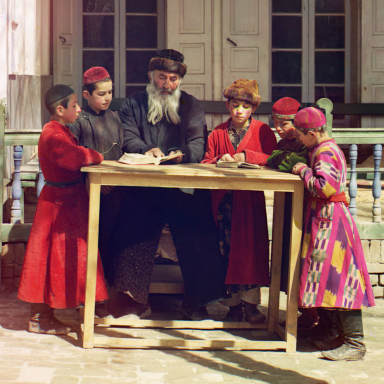
\includegraphics[width=0.3\textwidth]{f/samarkand.png} &
			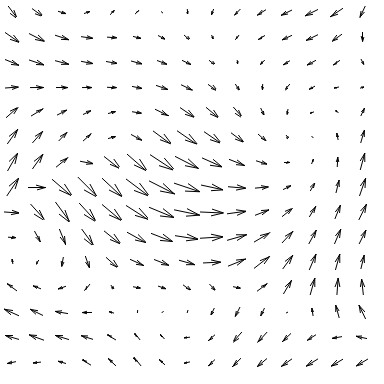
\includegraphics[width=0.3\textwidth]{f/deformation.png} &
			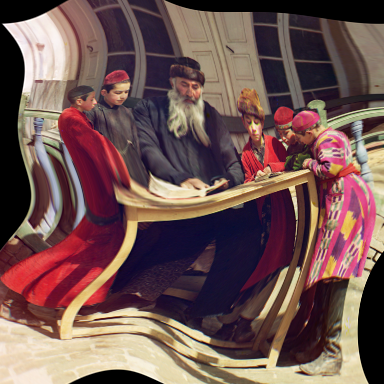
\includegraphics[width=0.3\textwidth]{f/deforkand.png} \\
			%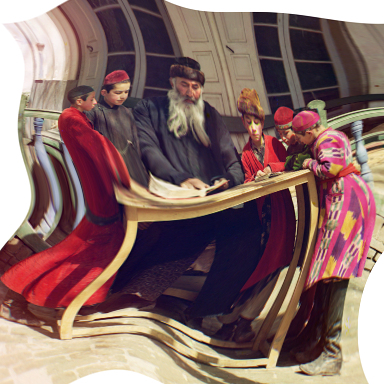
\includegraphics[width=0.3\textwidth]{f/ndeforkand.png} \\
			$A$ & $\u$ & $A\boxplus\u$ \\
		\end{tabular}
	\end{center}
	\caption{
	Push-forward of an image by a vector field.
	Notice that performing this computation requires the inversion of the vector
	field, which is a nonlinear iterative procedure.
	}
	\label{fig:pushforward}
\end{figure}

\section{Algorithm}

The pseudo-code below describes in detail the centroid method for the
correction of turbulence.  The ``main'' function
is~\texttt{CentroidCombination} which combines the centroids computed from
seven reference frames; this function is a computationally practical version
of formula~\ref{eq:Irecentroid}.

The core algorithm is the subroutine~\texttt{CentroidFromReference}, which is
simply the transcription of formula~(\ref{eq:Icentroid}).
The subroutine~\texttt{OpticalFlow}$(A,B)$ shall compute a vector field~$\u$
such that~$A\boxplus\u=B$ approximately.  In our case, we use the
Horn--Schunck method~\cite{horn1981determining} implemented in
IPOL~\cite{HSipol}, but this can be replaced by any other optical flow
technique.

The subroutine~\texttt{PushForward}$(A,\u)$ computes the image~$A\boxplus\u$.
This computation requires the inversion of a vector field, which is
performed by the function~\texttt{InvertField}.  The inversion of a vector
field~$\u$ is defined as a vector field~$\v$ such that if
\[
\varphi(\x):=\x+\u(\x)
\]
then
\[
\varphi^{-1}(\x)=\x+\v(\x).
\]
\par
We propose an algorithm~\cite{chen2008} to compute~$\v(\x)$ which
consists in doing~$6$
recursive applications of the mapping~$F(\y)=-\u(\x+\y)$, whose fixed point
is~$\y=\v(\x)$.
For a fixed~$\x$,  locally the Lipschitz constant of this mapping is the operator norm of
the Jacobian matrix~$D\u(\x)$.
Thus, for the pixels~$\x$ where~$\|D\u(\x)\|<1$ holds,
%
%, which can be roughly bounded
%by~$|(\mathrm{div}\,\u)(\x)|$.  Thus, for the pixels~$\x$
%where~$|(\mathrm{div}\,\u)(\x)|<1$ 
the fixed-point iterations converge to the inverse vector field.

The subroutines~\texttt{PushForward} and~\texttt{InvertField} need to
interpolate images at sub-pixel positions, which is done by the
subroutine~\texttt{InterpolateImageAt}.  We propose to use bi-cubic
interpolation~\cite{keys1981cubic}, as implemented by
function~\texttt{BicubicInterpolationImage} on the appendix, but this can be
replaced by a higher-order spline.

\begin{algorithm}[H]
	%\caption{centroid method}
	\caption{\texttt{CentroidFromReference}}
	\label{alg:centroid}
	\dontprintsemicolon
	\SetKwInOut{Input}{Input}
	\SetKwInOut{Output}{Output}
	\SetKwFunction{OpticalFlow}{OpticalFlow}
	\SetKwFunction{PushForward}{PushForward}

	\Input{Images~$I_1,\cdots,I_N$}
	\Input{Parameter~$r\in\{1,\ldots,N\}$, index of the reference image}
	\Output{Image~$I$}
	\BlankLine
	\For{$n=1,\ldots,N$}{
		$\u_n\leftarrow\OpticalFlow(I_r,\ I_n)$\;
	}
	\BlankLine
	$\u\leftarrow\displaystyle\frac{1}{N}\sum_{n=1}^N\u_n$\;
	\BlankLine
	$I\leftarrow\PushForward(I_r,\ \u)$\;
\end{algorithm}

\begin{algorithm}[H]
	\caption{\texttt{PushForward}}
	\label{alg:pushforward}
	\dontprintsemicolon
	\SetKwInOut{Input}{Input}
	\SetKwInOut{Output}{Output}
	\SetKwFunction{InvertField}{InvertField}
	\SetKwFunction{WIDTH}{WIDTH}
	\SetKwFunction{HEIGHT}{HEIGHT}
	\SetKwFunction{InterpolateImageAt}{InterpolateImageAt}

	\Input{Image~$I$}
	\Input{Vector field~$\u$}
	\Output{Image~$J=I\boxplus\u$}
	\BlankLine
	$\v\leftarrow\InvertField(\u)$\;
	%\For{$\x\in\{1,\ldots\WIDTH\}\times\{1,\ldots\HEIGHT\}$}{
	\For{$\x\in\Omega$}{
		%$\y\leftarrow\x+\v(\x)$\;
		$J(\x)\leftarrow\InterpolateImageAt(I,\ \x+\v(\x))$\;
	}
\end{algorithm}

\begin{algorithm}[H]
	\caption{\texttt{InvertField}}
	\label{alg:invertfield}
	\dontprintsemicolon
	\SetKwInOut{Input}{Input}
	\SetKwInOut{Output}{Output}
	\SetKwFunction{WIDTH}{WIDTH}
	\SetKwFunction{HEIGHT}{HEIGHT}
	\SetKwFunction{InterpolateImageAt}{InterpolateImageAt}

	\Input{Vector field~$\u$}
	\Output{Vector field~$\v$}
	\BlankLine
	%$\v=-\u$\;
	$\v=0$\;
	\For{$i=1,\ldots,6$}{
		%\For{$\x\in\{1,\ldots\WIDTH\}\times\{1,\ldots\HEIGHT\}$}{
		\For{$\x\in\Omega$}{
			$\v(\x)\leftarrow-\InterpolateImageAt(\u,\ \x+\v(\x))$\;
			%$\y\leftarrow\x+\v(\x)$\;
			%$\z\leftarrow\InterpolateImageAt(\u,\ \y)$\;
			%$\v(\x)\leftarrow-\z$\;
		}
	}
\end{algorithm}

\begin{algorithm}[H]
	\caption{\texttt{CentroidCombination}}
	\label{alg:centroidcombination}
	\dontprintsemicolon
	\SetKwInOut{Input}{Input}
	\SetKwInOut{Output}{Output}
	\SetKwFunction{CentroidFromReference}{CentroidFromReference}
	\SetKwFunction{GeometricMedian}{GeometricMedian}

	\Input{Images~$I_1,\cdots,I_N$}
	\Output{Image~$I$}
	\BlankLine
	$M\leftarrow 7$\;
	\For{$i=1,\ldots,M$}{
		$r\leftarrow 1+\lfloor N/M\rfloor(i-1)$\;
		$J_i\leftarrow\CentroidFromReference(I_1,\ldots,I_n,\ r)$\;
	}
	$I\leftarrow\GeometricMedian(J_1,\ldots,J_M)$\;
\end{algorithm}

\section{Results}

It is notoriously difficult to find freely available video sequences with a
high degree of turbulence in order to try these algorithms.  Since the
correction of videos degraded by turbulence has
military~\cite{maogilles2012,micheli2013} or sensitive~\cite{edf}
applications, the original sequences used to evaluate published methods are
typically not available.  In order to evaluate our online implementation we
use two video sequences available in the literature from the publications by
Efros et~al.~\cite{efros2005} and Tian et~al.~\cite{tian2009seeing}.  We also
use synthetic sequences produced by deforming a color photograph by smooth
random fields.

Figures~\ref{fig:expcvv} through~\ref{fig:expsim} show the results of the
function~\texttt{CentroidCombination} for these sequences.  See the on-line
demo associated to this article for a larger collection of experiments.
Notice that in general the method is always a clear improvement over the
average image.  The main advantage of the centroid method is that it can yield
useful results with a small amount of input frames (as opposed to
deconvolution-based methods, which need a large quantity of input images).  In
fact, the centroid of two deformed images is well-defined, and it exhibits
less deformation than either image.


% It is notoriously difficult to obtain test sequences for underwater
% turbulence, which is the kind of turbulence which is better sui

% small paragraph discussing the results
% description of the input sequences
% description of the results for each sequence
% for more visual results, see the demo
% comment table of numerical results

% sequences:
% 1. CVV 384
% 2. Video font tiny
% 3. Synthetic Samarkand "4,7", 400 frames
% 4. Synthetic Samarkand "4,7", 7 frames
% 5. Synthetic Samarkand "lblur", 400 frames

% figures showing the results. For each figure, 3 images:
% I1, Iavg, Icentroid

% table showing the error with respect to the ground truth in RMSE and MAE
% I1, Iavg, Imed, Icentroid, Ideconv


\begin{figure}[p]
	\begin{center}
		\begin{tabular}{ccc}
			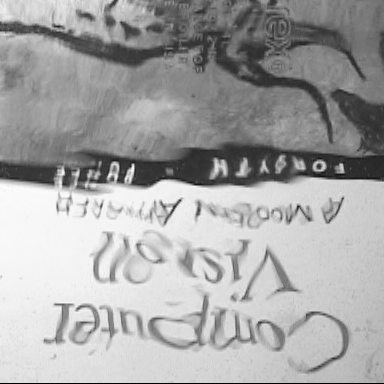
\includegraphics[width=0.3\textwidth]{f/cvv_first.png} &
			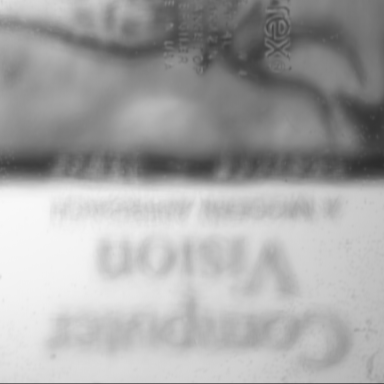
\includegraphics[width=0.3\textwidth]{f/cvv_avg.png} &
			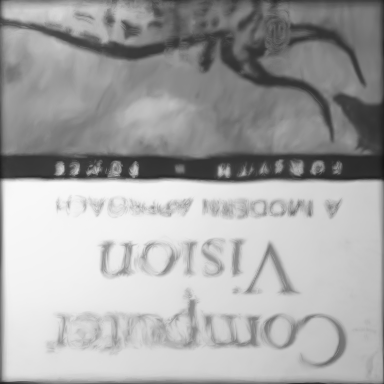
\includegraphics[width=0.3\textwidth]{f/cvv_centroid.png} \\
			$I_1$ & average & centroid \\
		\end{tabular}
	\end{center}
	\caption{Result of the centroid method for the sequence from
	reference~\cite{efros2005} (used with permission).
	This is an extract of~$400$ frames from the original sequence, cropped
	around the center of the image.
	}
	\label{fig:expcvv}
\end{figure}

\begin{figure}[p]
	\begin{center}
		\begin{tabular}{ccc}
			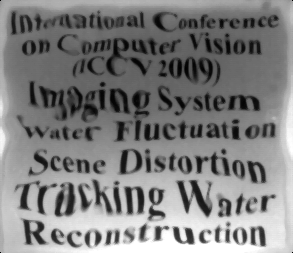
\includegraphics[width=0.3\textwidth]{f/tian_first.png} &
			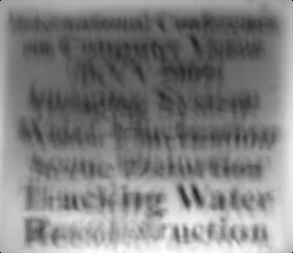
\includegraphics[width=0.3\textwidth]{f/tian_avg.png} &
			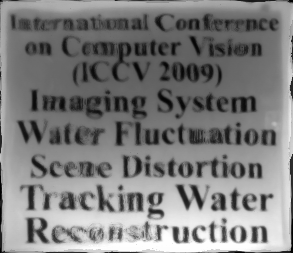
\includegraphics[width=0.3\textwidth]{f/tian_centroid.png} \\
			$I_1$ & average & centroid \\
		\end{tabular}
	\end{center}
	\caption{Result of the centroid method for the sequence from
	reference~\cite{tian2009seeing} (used with permission).
	This is a short sequence of~$61$ frames with rather large deformations,
	for which the average has not converged to a uniformly blurry image.
	}
	\label{fig:exptian}
\end{figure}

\begin{figure}[p]
	\begin{center}
		\begin{tabular}{ccc}
			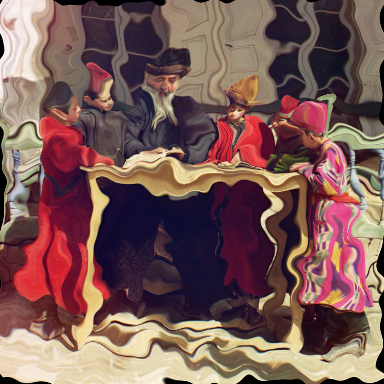
\includegraphics[width=0.3\textwidth]{f/sim_first.png} &
			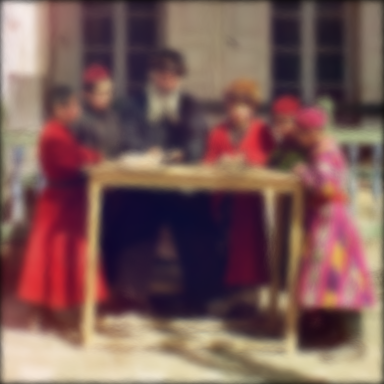
\includegraphics[width=0.3\textwidth]{f/sim_avg.png} &
			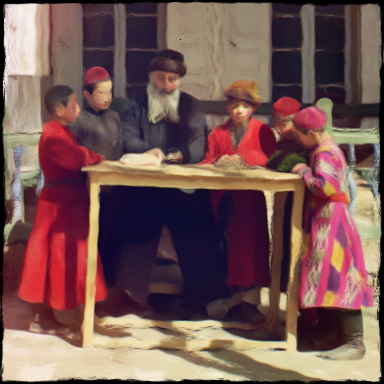
\includegraphics[width=0.3\textwidth]{f/sim_centroid.png} \\
			$I_1$ & average & centroid \\
		\end{tabular}
	\end{center}
	\caption{Result of the centroid method over a simulated sequence of~$400$
	frames.}
	\label{fig:expsim}
\end{figure}

%\begin{figure}[p]
%	\begin{center}
%		\begin{tabular}{ccc}
%			\includegraphics[width=0.3\textwidth]{f/sim7_first.png} &
%			\includegraphics[width=0.3\textwidth]{f/sim7_avg.png} &
%			\includegraphics[width=0.3\textwidth]{f/sim7_centroid.png} \\
%			$I_1$ & average & centroid \\
%		\end{tabular}
%	\end{center}
%	\caption{Result of the centroid method over a simulated sequence of~$7$
%	frames.}
%	\label{fig:expsim7}
%\end{figure}
%
%\begin{figure}[p]
%	\begin{center}
%		\begin{tabular}{ccc}
%			\includegraphics[width=0.3\textwidth]{f/simlblur_first.png} &
%			\includegraphics[width=0.3\textwidth]{f/simlblur_avg.png} &
%			\includegraphics[width=0.3\textwidth]{f/simlblur_centroid.png} \\
%			$I_1$ & average & centroid \\
%		\end{tabular}
%	\end{center}
%	\caption{Result of the centroid method over a simulated sequence of~$400$
%	frames with local blurs.}
%	\label{fig:explblur}
%\end{figure}

\clearpage

\section*{Appendix: Bicubic interpolation and vector medians}

This appendix describes the implementation of some auxiliary functions that
are needed in the rest of the algorithm.  The bicubic interpolation is used
for warping images and fields, and the Weiszfeld vector median can be,
optionally, used to combine several centroids as an alternative to
formula~\ref{eq:Irecentroid}.

\begin{algorithm}[hp]
	\caption{\texttt{BicubicInterpolationImage} (example
	of~\texttt{InterpolateImageAt})}
	\label{alg:bicubicinterpolationimage}
	\dontprintsemicolon
	\SetKwInOut{Input}{Input}
	\SetKwInOut{Output}{Output}
	\SetKwFunction{BicubicInterpolationCell}{BicubicInterpolationCell}

	\Input{Image~$I$}
	\Input{Position~$(x,y)$ inside the image domain}
	\Output{Value~$z$}
	\BlankLine
	$x\leftarrow x-1$\;
	$y\leftarrow y-1$\;
	\For{$i,j=0,1,2,3$}{
	%\For{$i=0,1,2,3$}{
	%\For{$j=0,1,2,3$}{
	$c_{ij}\leftarrow I\left(\lfloor x\rfloor+i,\ \lfloor y\rfloor+j\right)$\;
	%}}
	}
	$z\leftarrow\BicubicInterpolationCell(c,\ x-\lfloor x\rfloor,\ y-\lfloor
	y\rfloor)$\;
\end{algorithm}

\begin{algorithm}[hp]
	\caption{\texttt{BicubicInterpolationCell}}
	\label{alg:bicubicinterpolationcell}
	\dontprintsemicolon
	\SetKwInOut{Input}{Input}
	\SetKwInOut{Output}{Output}
	\SetKwFunction{CubicInterpolationLine}{CubicInterpolationLine}

	\Input{Sixteen cell values~$c_{ij},\quad i,j=0,1,2,3$}
	\Input{Position~$(x,y)$ inside the cell, $0\le x,y<3$}
	\Output{Value~$z$}
	\BlankLine
	%$v_0\leftarrow\CubicInterpolationLine(c_0,\ y)$\;
	%$v_1\leftarrow\CubicInterpolationLine(c_1,\ y)$\;
	%$v_2\leftarrow\CubicInterpolationLine(c_2,\ y)$\;
	%$v_3\leftarrow\CubicInterpolationLine(c_3,\ y)$\;
	%$z\leftarrow\CubicInterpolationLine(v,\ x)$\;
	$v_0\leftarrow\CubicInterpolationLine(c_{00},c_{01},c_{02},c_{03},\ y)$\;
	$v_1\leftarrow\CubicInterpolationLine(c_{10},c_{11},c_{12},c_{13},\ y)$\;
	$v_2\leftarrow\CubicInterpolationLine(c_{20},c_{21},c_{22},c_{23},\ y)$\;
	$v_3\leftarrow\CubicInterpolationLine(c_{30},c_{31},c_{32},c_{33},\ y)$\;
	$z\leftarrow\CubicInterpolationLine(v_0,v_1,v_2,v_3,\ x)$\;
\end{algorithm}

\begin{algorithm}[hp]
	\caption{\texttt{CubicInterpolationLine}}
	\label{alg:cubicinterpolationline}
	\dontprintsemicolon
	\SetKwInOut{Input}{Input}
	\SetKwInOut{Output}{Output}
	\SetKwFunction{BicubicInterpolationLine}{BicubicInterpolationLine}

	\Input{Four line values~$v_i,\quad i=0,1,2,3$}
	\Input{Position~$x$, $0\le x<3$}
	\Output{Value~$y$}
	\BlankLine
	$\setlength\delimitershortfall{-1pt}y\leftarrow v_1 +
	\frac{1}{2}\cdot x\cdot\left(v_2 - v_0
			+ x\cdot\left(2v_0 - 5v_1 + 4v_2 - v_3
			+ x\cdot\left(3(v_1 - v_2) + v_3 - v_0\right)\right)\right)$\;
	%$y\leftarrow 3(v_1-v_2)+v_3-v_0$\;
	%$y\leftarrow x\cdot y+2v_0-5v_1+4v_2-v_3$\;
	%$y\leftarrow x\cdot y+v_2-v_0$\;
	%$y\leftarrow 0.5\cdot x\cdot y+v_1$\;
\end{algorithm}

\begin{algorithm}[hp]
	\caption{\texttt{GeometricMedian} (Weiszfeld's algorithm)}
	\label{alg:weiszfeld}
	\dontprintsemicolon
	\SetKwInOut{Input}{Input}
	\SetKwInOut{Output}{Output}
	%\SetKwFunction{SmoothDistance}{SmoothDistance}

	\Input{A set of~$N$ $D$-dimensional vectors~$\x_1,\ldots,\x_N$}
	\Output{The geometric median~$\y$}
	\BlankLine
	$\varepsilon=10^{-3}$\;
	$\y\leftarrow\displaystyle\frac{1}{N}\sum_{n=1}^N\x_n$\;
	\For{$i=1,\ldots,5$}{
		$\y\leftarrow\displaystyle\frac
		{\displaystyle\sum_{n=1}^N \x_n
		/\sqrt{\varepsilon^2+\left\|\y-\x_n\right\|^2}}
		{\displaystyle\sum_{n=1}^N  1   /\sqrt{\varepsilon^2+\left\|\y-\x_n\right\|^2}}
		$\;
		%$\a\leftarrow\mathbf{0}$\;
		%$b\leftarrow0$\;
		%\For{$n=1,\ldots,N$}{
		%	$d\leftarrow\sqrt{\varepsilon^2+\left\|\y-\x_n\right\|_2^2}$\;
		%	%$d\leftarrow\SmoothDistance(\x_n,\ \y)$\;
		%	$\a\leftarrow\a+\x_n/d$\;
		%	$b\leftarrow b+1/d$\;
		%}
		%$\y\leftarrow\a/b$\;
	}
\end{algorithm}

%\begin{algorithm}[H]
%	\caption{\texttt{SmoothDistance}}
%	\label{alg:smoothdistance}
%	\dontprintsemicolon
%	\SetKwInOut{Input}{Input}
%	\SetKwInOut{Output}{Output}
%
%	\Input{Two $D$-dimensional vectors~$\x$ and~$\y$}
%	\Output{The smoothed distance~$b>\varepsilon$}
%	\BlankLine
%	$\varepsilon=10^{-4}$\;
%	$b\leftarrow\sqrt{\varepsilon^2+\sum_{d=1}^D(x_d-y_d)^2}$\;
%
%\end{algorithm}



%
% REFERENCES
%

\clearpage
\bibliographystyle{plain}
\bibliography{bibtex}


\end{document}

% vim: tw=78 sw=4 ts=4 spell spelllang=en:
